\documentclass{beamer}

% Thème
\usetheme{metropolis} % Un thème moderne
\usecolortheme{dove} % Couleurs épurées

% Paquets supplémentaires
\usepackage{graphicx}
\usepackage{booktabs}
\usepackage[french]{babel}

% Required package
\usepackage[absolute,overlay]{textpos}

\usepackage{fontspec}
\setmainfont{Helvetica}

% Informations sur la présentation
\title{1924B Mini Boîte Noire}
\subtitle{Enregistreur de données de vol}
\author{Ali Zoubir}
\institute{\textbf{ETML-\textcolor{red}{ES}}}
\date{\today}

\begin{document}
	
\begin{frame}[plain]
	\maketitle
	\begin{textblock*}{2cm}(9cm,5cm) % {block width} (coords)	
		\includegraphics[width=1\linewidth]{../figures/AMPA}
	\end{textblock*}
	\begin{textblock*}{2cm}(9cm,6.5cm) % {block width} (coords)	
		
\includegraphics[width=1\linewidth]{../figures/ETML-ES}
	\end{textblock*}
\end{frame}

\begin{frame}{Sommaire}
	\tableofcontents
\end{frame}

\section{Introduction}

\begin{frame}{Introduction}	
	\begin{textblock*}{4cm}(1cm,1cm) % {block width} (coords)	
	\begin{figure}[h]
		\centering
		\includegraphics[width=1\linewidth]{../figures/boite-noire}
		\caption{Boîte noire}
		\label{fig:boite-noire}
	\end{figure}
	\end{textblock*}
	
	\begin{textblock*}{7cm}(5.5cm,1.5cm) % {block width} (coords)
		Les enregistreurs de données de vol jouent un rôle crucial dans la sécurité aérienne et la compréhension des phénomènes aéronautiques en capturant de manière inaltérable des informations vitales. 
		
		Ce projet a pour but la collecte et le stockage des données de mesures et de \textcolor{blue}{localisation} d'un aéronef au moyen d'une centrale \textcolor{blue}{inertielle} et d'un système de positionnement GPS/GNSS.		
	\end{textblock*}
\end{frame}

\begin{frame}{Principe}	
	\begin{textblock*}{4.5cm}(1cm,1cm) % {block width} (coords)
	\begin{figure}[h]
		\centering
		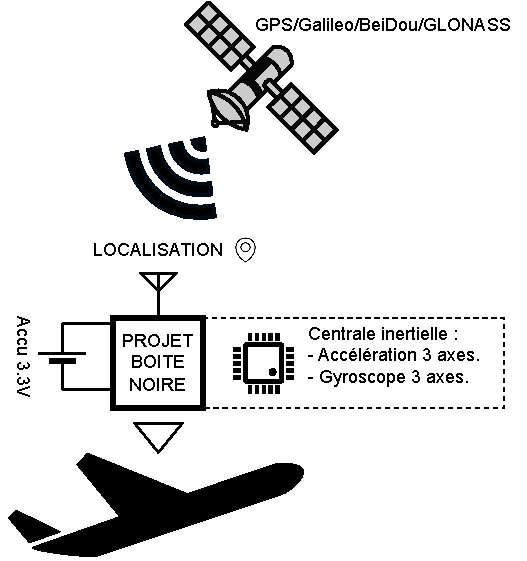
\includegraphics[width=1\linewidth]{../figures/cdc/schema_principe}
		\caption{Schéma de principe.}
		\label{fig:schemaprincipe}
	\end{figure}
	\end{textblock*}

	\begin{textblock*}{7cm}(5.5cm,1.5cm) 
	\begin{itemize}
		\item Données de localisation, trajectoire.
		\item Accéléromètre et Gyroscope.
		\item Miniaturisation.
		\item Bonne autonomie / Low power.
		\item Configuration des temps de sauvegardes.
		\item Charge, lecture et configuration par USB-C.
	\end{itemize}
	\end{textblock*}
\end{frame}

\section{Pré-étude}
\begin{frame}{Schéma bloc}
	\begin{figure}[h]
		\centering
		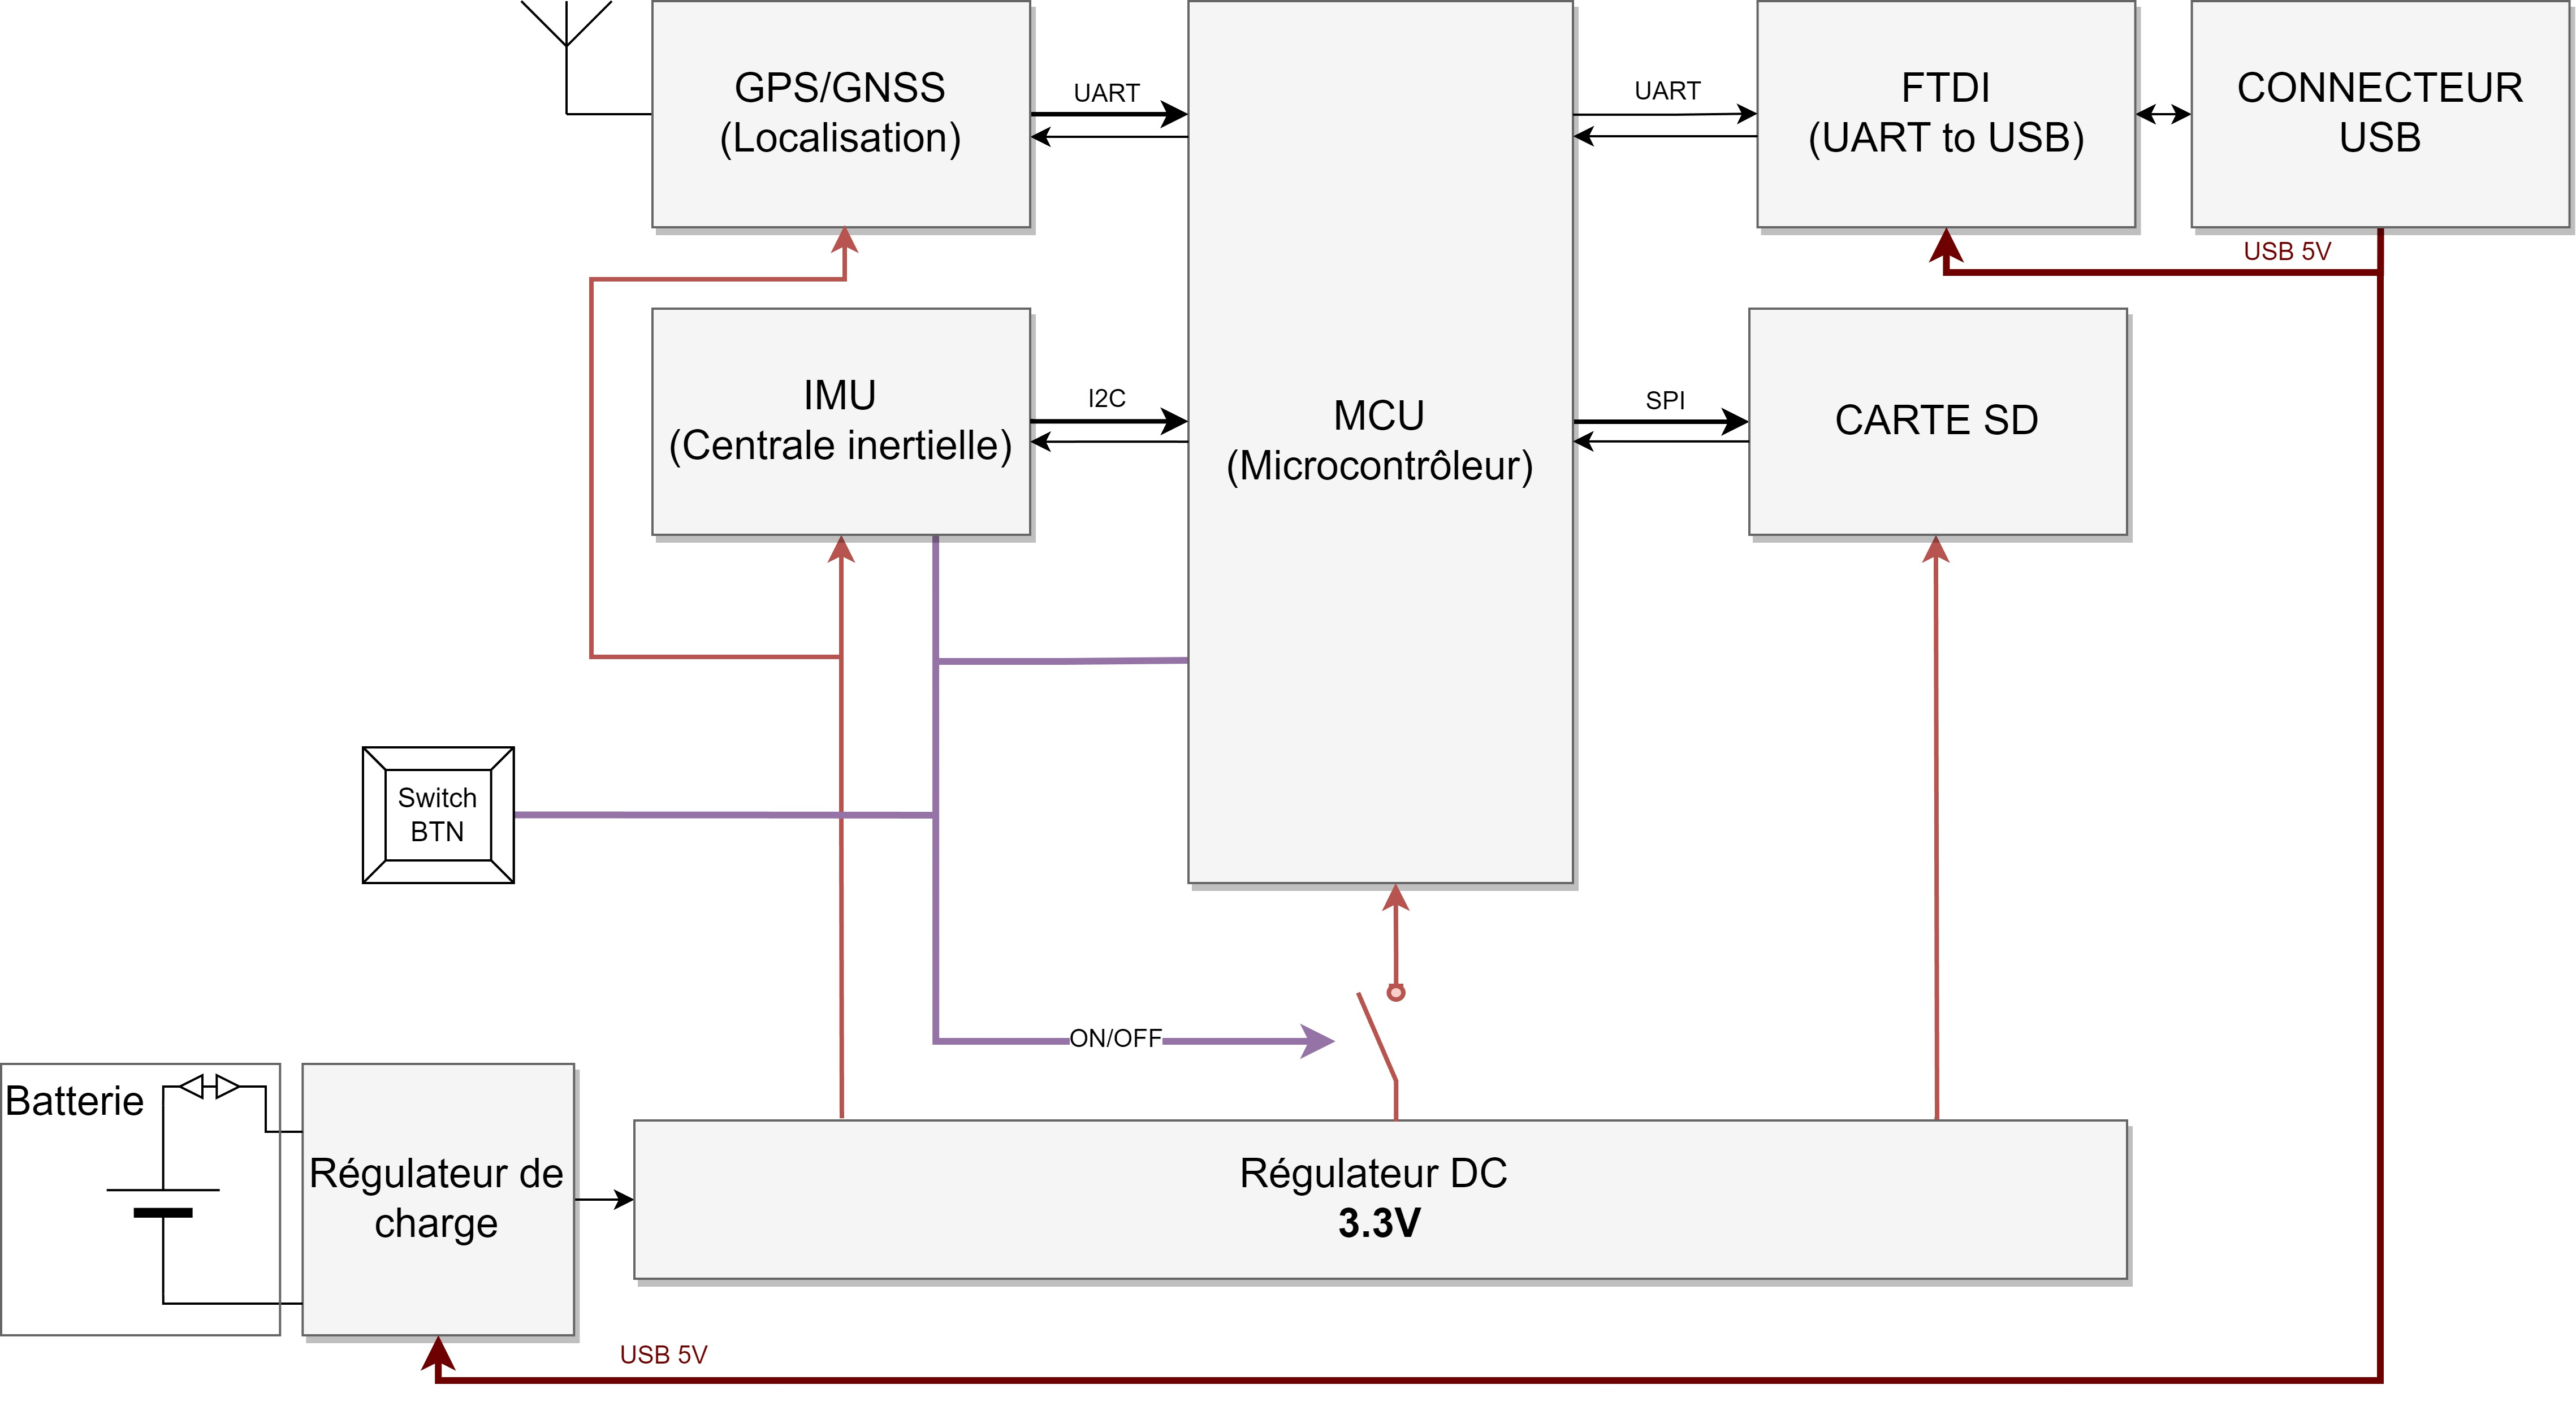
\includegraphics[width=1\textwidth]{../figures/cdc/blocs_grossiers_no_antenna}
		\caption{Schéma bloc.}
		\label{fig:schbloc}
	\end{figure}
\end{frame}

\begin{frame}{Choix des composants clés}
	\begin{tabular}{lll}
		Microcontrôleur &:& PIC32MX274F256D \\
		Centrale inertielle &:& BNO055 \\
		GNSS &:& CAM-M8C-0 \\
		Carte SD &:& 256MB \\
		Batterie &:& LI-ION \\
		Régulateur &:& MCP73871T-2CCI/ML\\
	\end{tabular}
\end{frame}

\section{Conclusion}
\begin{frame}{Conclusion}
	Résumons ce que nous avons appris.
\end{frame}

\begin{frame}[standout]
	Questions?
\end{frame}
	
\end{document}
